% =====================================================================
% Preamble --- IEEE Transactions on Affective Computing
%
% This replaces the single-column `article` layout used for the bioRxiv/arXiv
% preprint (kept at archive/preamble_preprint_2026-08.tex). IEEE Computer
% Society states without qualification that template use is mandatory for
% journal submissions, so the class, the bibliography style and the float
% handling are all fixed by the template rather than chosen:
%
%   https://www.computer.org/publications/author-resources
%     "Journals: Using an article template is required for journal submissions."
%   https://www.computer.org/csdl/journal/ta/write-for-us/15060
%     "Regular paper - 12 double column pages (Submissions may be up to 18
%      pages in length, subject to MOPC.)"
%
% Two page numbers therefore matter and are not the same thing. Twelve pages
% is the Mandatory Overlength Page Charge threshold ($220 for each page or
% fraction beyond it); EIGHTEEN is the hard cap on what may be submitted at
% all. The preprint ran to 40 single-column pages, which is roughly 25 in this
% layout, so the conversion is a compression job as much as a reformatting one:
% the long figure legends moved into the Supplementary Information, which TAC
% explicitly does not cap, and the Methods keep only what a reader needs to
% judge the result.
%
% Line numbering: the preprint carried a \iflinenums switch because arXiv puts
% submissions with margin line numbers on hold. IEEEtran has no such
% requirement and ScholarOne does not ask for them, so the switch is gone.
% =====================================================================
\documentclass[journal]{IEEEtran}

\usepackage[T1]{fontenc}
\usepackage[utf8]{inputenc}
\usepackage{microtype}

\usepackage{amsmath,amssymb}
\usepackage{graphicx}
\usepackage{booktabs}
\usepackage{multirow}
\usepackage{array}
\usepackage{url}
\usepackage[hidelinks]{hyperref}
\usepackage{xcolor}

% IEEEtran wants its own citation handling; cite.sty gives the sorted,
% compressed [3]--[5] form the journal uses.
\usepackage{cite}
\bibliographystyle{IEEEtran}

% Two-line table headers. Several tables have column headings far wider than
% the numbers beneath them, which in two columns runs the table past the
% measure; stacking the heading makes each column as wide as its data.
\newcommand{\thd}[2]{\begin{tabular}[b]{@{}c@{}}#1\\#2\end{tabular}}

\usepackage{upgreek}
\newcommand{\uV}{\ensuremath{\upmu\mathrm{V}}}

% ORCID iD as the linked green icon IEEE now sets after an author's name.
% Only J. Zhang has one; X. Yao does not, and an author without an ORCID simply
% carries no icon -- nothing is left blank and nothing is invented.
\usepackage{orcidlink}

% Shorthand for the two variants of the environmental corpus that the
% mixture-leakage control forces us to distinguish everywhere (Section
% III-C). Spelling them out each time costs a line per occurrence.
\newcommand{\emoAll}{Emo-Soundscapes (all 1{,}213)}
\newcommand{\emoOrig}{Emo-Soundscapes (600 originals)}

\hyphenation{op-tical net-works semi-conduc-tor}


\renewcommand{\thesection}{S\arabic{section}}
\renewcommand{\thefigure}{Extended Data Figure~\arabic{figure}}
\renewcommand{\thetable}{S\arabic{table}}
\captionsetup[figure]{labelformat=empty}

\title{\bfseries Supplementary Information\\[2mm]
\large Not all generalisation failures can be bought back:
four boundaries in affective audio modelling}

\begin{document}
\maketitle

\tableofcontents
\clearpage

% =====================================================================
% A "How this document is organised" section stood here. It was four paragraphs
% that mostly restated two things the reader already had: the main text's three
% quantities, and the table of contents on the previous page. What was genuinely
% its own -- that Sections S1--S6 are load-bearing rather than context, and that
% each follows a fixed four-part structure -- is one sentence, kept below; the
% rest of it duplicated the caption of Table S1 immediately underneath. It also
% cost a table-of-contents entry that said only "how this document is organised",
% which is noise in a nine-entry list.

Sections~S1--S6 are admission criteria: checks that had to pass before a main-text
claim was allowed to be made, each reported in the same four parts --- what was
checked, the decision rule fixed before the check, the outcome, and the claim the
outcome licenses. Sections~S7--S9 then cover the representation-family extraction,
the withdrawn analyses, and the Extended Data figures.

\begin{table}[htbp]
\centering\small
\caption{The six admission criteria and the main-text claims they license. A criterion
that failed removes a claim rather than weakening it; two of the six did fail, and the
corresponding analyses are absent from the main text rather than reported as null
results.}
\begin{tabular}{p{1.0cm}p{5.8cm}p{7.2cm}}
\toprule
Section & What had to pass & What the outcome licenses \\
\midrule
S1 & The documented mapping from stimulus trigger code to audio file in ds002721 must
reproduce, or be recoverable against a permutation null.
& \textbf{Failed.} No acoustic-to-physiological analysis is reported in that corpus.
Its trigger codes are used only as stimulus identifiers, for which their internal
consistency suffices. \\
\addlinespace
S2 & Both pre-declared electrodermal positive controls must pass, applied at the level
at which the conclusion would be drawn.
& \textbf{Failed.} The corpus and its conclusion are withdrawn. The physiological
negatives that remain in the main text are the ones whose instrument was shown to
work. \\
\addlinespace
S3 & Loudness must not act as a corpus identifier before descriptors are computed; and
the physiological null must not be an artefact of having removed loudness.
& Boundary~1, the domain wall (Fig.~1 and Table~1); Boundary~3, the physiological
ceiling. \\
\addlinespace
S4 & The reliability of each target must be estimated, with a stated estimator, before
any percentage of it is quoted.
& The denominator of every survival fraction at all four boundaries, including the
84\% within corpus and the 31\% bound on the physiological target. \\
\addlinespace
S5 & A within-song correlation between two autocorrelated series must exceed a
circular-shift null before it is called a coupling.
& That all four boundaries are stated at the level of the excerpt, and that
moment-to-moment modulation is a separate and much smaller quantity. \\
\addlinespace
S6 & A cross-model attribution consensus must exceed its label-permutation reference
distribution before it is treated as a stable descriptor set.
& \textbf{Failed.} Transfer is measured at every boundary and never inferred from
which descriptors a model relies on within its own corpus (Fig.~2). \\
\bottomrule
\end{tabular}
\end{table}

\clearpage
% =====================================================================
\section{Admission criterion: the trigger-to-audio mapping in ds002721}

Two errors in the event annotation of this dataset were found while preparing the
analyses in the main text, and both would affect anyone reusing it. We report them so
that the corrections are available, and we have written to the dataset authors. The
second is the admission criterion for Boundary~3: it determines which questions this
corpus can be asked.

\subsection{The documented response codes are not the response}

\paragraph{What was checked.}
\texttt{events.json} documents two code families as both encoding a 1--9 rating:
\texttt{833--841} (``Response 01--09'') and \texttt{901--909} (``Answer 01--09'').
They agree on only \textbf{7.3\%} of trials, so at most one can be the rating.

\paragraph{Decision rule.}
The question can be settled without any external reference, using the internal
structure of the eight emotion scales. Ratings of pleasantness and happiness must
covary positively; pleasantness and fear negatively; anger and fear positively. The
encoding that reproduces the expected sign on the twelve relations is the rating; if
neither did, no rating analysis would be reported.

\begin{table}[htbp]
\centering\small
\caption{Internal structure of the eight emotion scales under each candidate
response encoding.}
\begin{tabular}{lcc}
\toprule
Expected relation & \texttt{833--841} & \texttt{901--909} \\
\midrule
pleasant $\leftrightarrow$ happy, positive  & $-0.015$ & $\mathbf{+0.503}$ \\
pleasant $\leftrightarrow$ tender, positive & $-0.173$ & $\mathbf{+0.519}$ \\
pleasant $\leftrightarrow$ afraid, negative & $+0.075$ & $\mathbf{-0.584}$ \\
angry $\leftrightarrow$ afraid, positive    & $+0.065$ & $\mathbf{+0.600}$ \\
happy $\leftrightarrow$ sad, negative       & $+0.077$ & $\mathbf{-0.299}$ \\
\midrule
six relations expected positive & mean $-0.063$, 2/6 & \textbf{mean $+0.406$, 6/6} \\
six relations expected negative & mean $+0.005$, 2/6 & \textbf{mean $-0.382$, 6/6} \\
\bottomrule
\end{tabular}
\end{table}

\paragraph{Outcome.}
\texttt{901--909} carries the ratings. \texttt{833--841} shows no coherent emotional
structure. All rating analyses in the main text use \texttt{901--909}.

A second, smaller point: the question codes \texttt{800--807} are re-emitted when a
question is redisplayed, so a rating must be matched to the nearest question code
within a tolerance rather than by exact timestamp equality. Exact matching drops
roughly 45\% of ratings.

\subsection{The stimulus codes do not resolve to the documented audio files}

\paragraph{What was checked.}
\texttt{events.json} states that stimulus codes span 301--360 and that subtracting
300 gives the filename. The observed codes span \textbf{302--657}, exactly ten per
music run, strictly interleaved with the fixation and music-onset markers. Assuming
the codes are $\mathrm{stimulus} + 300$ yields indices into the published stimulus
set that do not correspond to what participants reported:

\begin{itemize}
\item Participants' eight ratings against the published mean ratings of the mapped
clips: all 64 pairings, $|\rho| \le 0.16$.
\item A spectral-centroid probe against published ``energy'' ratings:
$\rho = +0.37$.
\item The same probe against participants' ``energetic'' ratings:
$\rho = -0.01$.
\end{itemize}

The codes are nevertheless genuine stimulus identities: participants who received
the same code agree strongly in their ratings (split-half $0.80$--$0.87$). The
numbering scheme, not the codes, is what is missing.

\paragraph{Decision rule.}
We attempted to recover the mapping by matching the eight-dimensional emotion profile
of each code against that of each published clip, optimising the assignment with the
Hungarian algorithm. The rule fixed in advance was that the recovered assignment must
beat a null formed by permuting stimulus labels within participant and regenerating
the profiles; otherwise the acoustic-to-physiological link would not be examined in
this corpus at all.

\paragraph{Outcome.}
The recovered assignment was not better than chance (observed mean profile correlation
$0.672$; null mean $0.654$, 95th percentile $0.681$; $p = 0.19$), and none of the
recovered pairings matched the documented rule.

\paragraph{What it licenses.}
\textbf{The acoustic-to-physiological link could not be examined in this corpus, and
is not examined in the main text.} What Boundary~3 reports instead is a comparison
between two response channels measured on the same trials --- what listeners say and
what their EEG does --- for which stimulus identity is sufficient and stimulus
\emph{content} is not required. Every use of these codes in the main text is as an
identifier only.

A third observation, possibly related: the dataset README describes participants as
hearing 40 clips, which would imply a common set. We observe 39--40 clips per
participant but \textbf{307 distinct codes across the 31 participants}, with a
median pairwise overlap of six clips. This is also the reason the stimulus-level
reliability estimator in the main text is the one appropriate to an unbalanced
design.

% =====================================================================
\section{Admission criterion: withdrawal of the electrodermal corpus}

An earlier version of this work analysed an electrodermal corpus
\citep{kutt2022} and reported that single-stimulus peripheral responses carry no
reproducible stimulus-level component. \textbf{That conclusion is withdrawn.} It
was not withdrawn because the effect exists; it was withdrawn because we could not
establish that the analysis pipeline could detect any effect at all.

\subsection{How it was found}

The reported conclusion conflicts with a well-established literature on
category-level skin-conductance responses to affective sounds. Prompted by that
conflict, we tested the pipeline against effects known to be present.

\begin{table}[htbp]
\centering\small
\caption{Group-level positive controls, under two implementations. The two share
their input recordings and their event timing and differ only in the decomposition
of the signal, so agreement between them bounds implementation error and is not
independent corroboration of the controls themselves.}
\begin{tabular}{lccc}
\toprule
Positive control & Expected & Hand-written & NeuroKit2 \\
\midrule
Habituation across trials & $\rho < 0$ & $\mathbf{+0.113}$, $p = 0.002$
  & $\mathbf{+0.101}$, $p = 0.015$ \\
Post-stimulus $>$ random window & significant & $p = 0.267$ & $p = 0.357$ \\
\bottomrule
\end{tabular}
\end{table}

Habituation was significant in the direction opposite to the established effect,
and stimulus locking was absent. Both held after replacing our implementation with
a published, validated toolbox \citep{makowski2021}.

\subsection{Five candidate explanations, all excluded}

\begin{table}[htbp]
\centering\small
\caption{Candidate explanations for the control failures, and their tests.}
\begin{tabular}{p{4.6cm}p{4.6cm}p{4.6cm}}
\toprule
Hypothesis & Test & Outcome \\
\midrule
Timestamp semantics (response time, not onset)
  & event-related average swept over $\pm16$\,s
  & no peak at any lag \\
Missing phasic decomposition
  & 0.05\,Hz high-pass added
  & reliability $-0.085 \rightarrow +0.110$; controls still fail \\
Ill-conditioned filter at 1\,kHz
  & decimate to 20\,Hz before filtering
  & $8.3 \times 10^{-7}$ vs $7.8 \times 10^{-7}$, no change \\
Implementation defect
  & replace with NeuroKit2
  & same failures \\
Unit scaling
  & rescale by $10^4$ and $10^5$
  & 66 responses detected at all three scalings \\
\bottomrule
\end{tabular}
\end{table}

The second row is itself a correction. The original extraction linearly detrended
within a 6\,s window, while the dominant variance in this signal is drift on the scale
of minutes; trial-level responses were buried rather than absent. After adding the
high-pass, stimulus-level reliability rose from $-0.085$ to $+0.110$ and the
category-level ordering became consistent with the literature. \textbf{The strong form
of the original claim --- that no reproducible stimulus-level component exists --- is
therefore withdrawn twice over}, once for the extraction defect and once for the
control failure below. What can be said is that per-stimulus reliability is low
($0.110$) against $0.750$ for the same participants' ratings of the same trials.

\subsection{The group-level verdict was itself tested}

\paragraph{Decision rule.}
A group mean in the wrong direction is compatible with a usable subset: if some
recordings failed technically, they could displace the mean while the remainder
stayed valid. This dataset's own publication documents extensive equipment problems,
so the possibility was concrete. We therefore applied both controls \emph{per
participant}, with each participant's own permutation null, and fixed the rule that
the corpus would be retained only if a subset of participants passed both.

\begin{table}[htbp]
\centering\small
\caption{Per-participant positive controls (94 analysable participants,
500 permutations each).}
\begin{tabular}{lcc}
\toprule
Per-participant control & Passing & Chance expectation \\
\midrule
Habituation ($\rho < 0$ and $p < 0.05$) & 8 / 94 & 4.7 \\
Stimulus locking ($p < 0.05$)           & 4 / 94 & 4.7 \\
\textbf{Both}                           & \textbf{0 / 94} & 0.24 \\
\bottomrule
\end{tabular}
\end{table}

\paragraph{Outcome.}
Decisively, habituation was in the expected direction for only \textbf{35\%} of
participants, where a working measurement would put it well above 50\%. The wrong
direction is therefore the majority behaviour, not a minority artefact displacing a
mean. No usable subset exists.

\paragraph{What it licenses.}
The corpus is excluded from every substantive analysis, and the main text reports the
exclusion rather than the negative result it would otherwise have produced. This is
what makes the remaining physiological results at Boundary~3 readable: the EEG corpus
that carries them passes four dataset-level controls and an individual-level control
before any reliability is estimated. A negative result from an instrument that has not
been shown to work is not a negative result.

\subsection{What we take from it}

Reliability testing and positive controls answer different questions and do not
substitute for one another. Testing whether a target variable carries reproducible
signal says nothing about whether the instrument works. We had performed the first
and omitted the second, and the omission produced a publishable-looking negative
result that we could not defend.

% =====================================================================
\section{Admission criterion: loudness normalisation}

Loudness enters this work twice, in opposite roles, and both had to be settled before
a main claim could be made. For the domain wall, absolute level is a corpus
\emph{identifier} that must be removed or the wall is measured against an inflated
baseline. For the physiological ceiling, absolute level is the most plausible
\emph{true} driver of an autonomic response, so having removed it is the most
obvious mundane explanation for a null and must be excluded.

\subsection{Loudness as a corpus fingerprint}

\paragraph{What was checked.}
All audio is loudness-normalised to $-23$\,LUFS (ITU-R BS.1770, integrated, gain
scaling only, no limiting) before any descriptor is computed. The check is whether
this changes cross-corpus transfer, using DEAM $\rightarrow$ PMEmo with five
classifiers, and whether it changes which descriptors the models use.

\paragraph{Decision rule.}
The rule was written in terms of the loss in transfer performance that normalisation
would cause, with three branches: a small loss would mean loudness carries genuine
shared signal; a large loss would mean the models had been learning loudness alone
and the descriptor work could not proceed; an intermediate loss would require a
per-corpus decision.

\paragraph{Outcome.}
Transfer performance \emph{rose}, which is a fourth case the rule did not cover. We
record that rather than reclassify it after the fact.

\begin{table}[htbp]
\centering\small
\caption{Loudness normalisation, DEAM $\rightarrow$ PMEmo. The first three rows are
out-of-corpus quantities and all improve; the fourth is a within-corpus sanity check
and falls slightly. The last row gives the mean rank, across models, of the strongest
absolute-level descriptor among the 122.}
\begin{tabular}{lccc}
\toprule
 & Raw & $-23$\,LUFS & $\Delta$ \\
\midrule
Cross-corpus AUC (random forest)      & 0.9180 & \textbf{0.9304} & $+0.0124$ \\
Cross-corpus recall (random forest)   & 0.4138 & 0.5172 & $+0.1034$ \\
Test excerpts inside the applicability domain & 78.0\% & 86.7\% & $+8.7$\,pp \\
Within-corpus cross-validated AUC     & 0.9378 & 0.9282 & $-0.0096$ \\
Mean attribution rank of \texttt{rms\_p90} (of 122) & 39.0 & 93.0 & $+54.0$ \\
\bottomrule
\end{tabular}
\end{table}

The mechanism is specific and checkable: DEAM is a mixed library and PMEmo consists of
pop choruses mastered at high level, so the two corpora differ in loudness
distribution before they differ in anything else. A model trained on the first learns
that loud means aroused and mis-calibrates on the second. Normalisation removes that
layer, which is why an out-of-corpus quantity improves while a within-corpus quantity
does not.

\paragraph{What it licenses.}
Every transfer number in Fig.~1 and Table~1, and the wall itself. Without
normalisation the same-domain transfer against which the cross-domain collapse is
measured is inflated by a corpus fingerprint, and the 59-to-74 percentage-point gap
between the two swaps could not be attributed to the domain boundary. It also carries
an engineering consequence stated in Methods: a deployed system must normalise before
scoring, or it reproduces the same fingerprint.

One semantic caution: \texttt{mfcc1\_mean} remains in the leading descriptors after
normalisation, but it no longer indexes absolute loudness --- it indexes spectral
tilt. It must not be read as a loudness rule.

\subsection{The physiological null does not depend on loudness having been removed}

\paragraph{What was checked.}
Normalisation removes a $6.7$-fold spread in across-track loudness, and sound level is
the best-established physical driver of electrodermal response. If the acoustic
descriptors fail to predict song-level electrodermal response only because we
discarded level, the physiological ceiling result would be an artefact of our own
preprocessing.

\paragraph{Decision rule.}
Three feature pipelines were compared on the same 717 songs, the same folds and the
same scoring: our descriptors on normalised audio, our descriptors re-extracted from
the original audio at its native loudness, and the 6{,}373-dimensional ComParE feature
set distributed with the corpus, which its authors extracted from the original audio
with an independent toolchain. A difference in best $\rho$ exceeding $0.05$ between
pipelines would mean the null is a preprocessing artefact.

\paragraph{Outcome.}
The three routes agree.

\begin{table}[htbp]
\centering\small
\caption{Song-level electrodermal prediction under three feature pipelines. The best
of six algorithms is reported for each. This is the only place in this work where a
claim rests on agreement between independently constructed pipelines.}
\begin{tabular}{llc}
\toprule
Pipeline & Audio & Best $\rho$ \\
\midrule
Hand-specified descriptors (normalised)   & $-23$\,LUFS & 0.045 \\
Hand-specified descriptors (re-extracted) & original loudness & 0.049 \\
ComParE, 6{,}373 features, extracted by the corpus authors & original loudness & 0.072 \\
\bottomrule
\end{tabular}
\end{table}

The spread is $0.027$, below the pre-declared $0.05$. Loudness used alone as a single
predictor reaches $+0.059$, which is within the same band.

\paragraph{What it licenses.}
The statement at Boundary~3 that no acoustic route reaches a usable fraction of the
attainable ceiling on the physiological target. It excludes the most plausible mundane
explanation for that null with one number.

\paragraph{A restriction on how agreement may be used elsewhere.}
This is the only surviving claim in this work of the form ``independently constructed
pipelines agree''. An earlier version used that form in several places, most of them
resting on attribution rankings shared between models, which Section~S6 shows is not
evidence of anything. No other analysis in the main text or this document should be
read as claiming convergence of independent paths.

% =====================================================================
\section{Admission criterion: the annotation reliability ceiling}

Every survival fraction in the main text is a ratio, and this section is its
denominator. A model that reaches $\rho = 0.77$ on a target whose own reproducible
component is $0.87$ has almost exhausted the target; the same $\rho$ on a target whose
reproducible component is $0.99$ has not. Without the denominator the four boundaries
cannot be compared with one another, and the comparison is the entire argument.

\paragraph{What was checked.}
The reliability of each target, estimated before any percentage of it was quoted, with
the same estimator applied to the physiological targets as to the ratings.

\paragraph{Estimator.}
Where per-rater judgements are released, reliability is estimated by splitting raters
at random into two halves, computing stimulus means within each half, correlating the
two sets of means and correcting to the full rater panel by the Spearman--Brown
formula; the reported value is the mean over 200 random splits, and we also report the
10th and 90th percentiles across splits because a ceiling estimated from ten raters
per stimulus is itself uncertain. For DEAM this uses 17{,}762 individual judgements
from 195 raters, with a median of ten per song.

Where only stimulus means and their across-observer standard deviations are released
--- PMEmo --- the same quantity is obtained analytically: the within-stimulus variance
is the mean of the squared across-observer standard deviations, the variance of the
stimulus mean is $\sigma^2_{\mathrm{between}} + \sigma^2_{\mathrm{within}}/n$, and the
single-observer intraclass correlation is stepped up to the $n$-observer mean by the
same Spearman--Brown expression. On the electrodermal targets, where per-listener
values \emph{are} available, both estimators were computed and agree
(analytic $0.146$--$0.350$ against split-half $0.138$--$0.232$), which is what
licenses the analytic form on the ratings side.

\begin{table}[htbp]
\centering\small
\caption{Reliability of every target used in this work, and the two denominators it
implies. $r$ is the reliability of the group-averaged target; $\sqrt{r}$ is the
largest correlation a perfect predictor could attain against the noisy target.
Brackets give the 10th and 90th percentiles over 200 rater splits for the DEAM
analysis subset, and 95\% confidence intervals for the two ds002721 rows, whose
estimator is an
intraclass correlation over trials rather than a corrected split-half and which is
therefore not directly comparable with the rows above it. Corpora that release no
per-rater or per-observer data admit no estimate; transfer into them is reported in
the main text as a raw correlation and never as a percentage.}
\begin{tabular}{p{5.2cm}p{4.4cm}cc}
\toprule
Target & Estimator & $r$ & $\sqrt{r}$ \\
\midrule
DEAM arousal, analysis subset ($n = 1{,}233$) & rater split-half, Spearman--Brown
  & \textbf{0.868} & 0.932 \\
\multicolumn{2}{l}{\quad \emph{10th--90th percentile over splits}}
  & [0.838, 0.889] & \\
DEAM arousal, all songs ($n = 1{,}802$) & rater split-half, Spearman--Brown
  & 0.837 & 0.915 \\
DEAM valence, all songs & rater split-half, Spearman--Brown & 0.792 & 0.890 \\
PMEmo arousal ($n = 717$) & analytic ICC, Spearman--Brown & 0.935 & 0.967 \\
PMEmo valence ($n = 717$) & analytic ICC, Spearman--Brown & 0.893 & 0.945 \\
ARAUS soundscape ratings & split-half on the 4.4\% of stimuli with two or more
  raters & 0.566 & 0.752 \\
IADS-sound ratings (BIRAFFE2) & listener split-half, Spearman--Brown
  & 0.750--0.813 & 0.866--0.902 \\
\midrule
PMEmo electrodermal, \texttt{phasic\_mean} & analytic ICC, Spearman--Brown
  & 0.350 & 0.592 \\
PMEmo electrodermal, \texttt{scl\_slope} & analytic ICC, Spearman--Brown
  & 0.285 & 0.534 \\
PMEmo electrodermal, \texttt{scr\_rate} & analytic ICC, Spearman--Brown
  & 0.146 & 0.382 \\
\midrule
ds002721 ratings, best of 8 scales & stimulus-level ICC, unbalanced design
  & 0.221 & --- \\
\multicolumn{2}{l}{\quad \emph{95\% confidence interval}} & [0.155, 0.281] & \\
ds002721 EEG, best of 156 measures & stimulus-level ICC, unbalanced design
  & 0.092 & --- \\
\multicolumn{2}{l}{\quad \emph{95\% confidence interval}} & [0.037, 0.142] & \\
\midrule
Emo-Soundscapes & no per-rater data released & --- & --- \\
Soundtracks & no per-rater data released & --- & --- \\
\bottomrule
\end{tabular}
\end{table}

\paragraph{Two denominators, and which is used where.}
A percentage of a ceiling is meaningless until the convention is named, because two
are in use and they differ by an amount that grows as reliability falls. Dividing by
$r$ answers ``what fraction of the reproducible variance in the target has been
recovered''. Dividing by $\sqrt{r}$ is the classical correction for attenuation and
answers ``what fraction of the largest attainable correlation has been reached''; it
is the more conservative of the two at low reliability, and it is the convention we
adopt wherever a physiological target is involved. On DEAM the two give 89\% and 83\%
for the same model; on an electrodermal target with $r = 0.146$ they differ by a
factor of $2.6$. \textbf{Main-text percentages against a rating target use $\rho/r$;
percentages involving a physiological target use $\rho/\sqrt{r}$, which is the
convention under which the $31\%$ bound is quoted.} Mixing the two within one
comparison --- which an earlier version of this work did, taking the subjective
percentage from one corpus under one convention and the physiological percentage from
another corpus under the other --- is a defect and is recorded as such in
Section~S8.

\paragraph{The homologous table.}
The comparison that Boundary~3 rests on was recomputed so that both sides come from
the same corpus, the same songs, the same features, the same folds and the same
reliability estimator. This is the table that supports the ceiling claim; the
per-corpus values above supply the denominators used elsewhere.

\begin{table}[htbp]
\centering\small
\caption{One ruler. The same 717 PMEmo songs, the same 161 descriptors, the same
artist-grouped folds and the same reliability estimator, applied to a rating target
and to three electrodermal targets. Achievement is $\rho/\sqrt{r}$ with a double
bootstrap interval.}
\begin{tabular}{lcccc}
\toprule
Target & $r$ & $\sqrt{r}$ & Acoustic $\rho$ & Achievement, 95\% CI \\
\midrule
Arousal (rating)  & 0.935 & 0.967 & 0.817 & \textbf{84.4\%} [81.5, 87.0] \\
Valence (rating)  & 0.893 & 0.945 & 0.705 & 74.6\% [70.4, 78.5] \\
EDA \texttt{phasic\_mean} & 0.350 & 0.592 & 0.032 & 5.4\% [$-6.8$, $+17.4$] \\
EDA \texttt{scl\_slope}   & 0.285 & 0.534 & 0.029 & 5.5\% [$-7.5$, $+18.8$] \\
EDA \texttt{scr\_rate}    & 0.146 & 0.382 & 0.014 & 3.7\% [$-15.2$, $+22.6$] \\
\bottomrule
\end{tabular}
\end{table}

The three physiological intervals all contain zero. The bound quoted in the main text
is not from this table but from the route comparison that follows it.

\paragraph{A correction to how that comparison was scored.} An earlier version
divided every route's correlation by a single ceiling, $\sqrt{r} = 0.592$, taken from
\texttt{phasic\_mean}. But the three electrodermal measures have different
reliabilities and therefore different ceilings --- $0.382$, $0.592$ and $0.534$ --- and
a route's best correlation is not always obtained on \texttt{phasic\_mean}. The first
acoustic principal component, for instance, reaches $\rho = 0.114$ against
\texttt{scl\_slope}, whose ceiling is $0.534$, and scoring it against $0.592$
understated it. This is the same mismatched-denominator error recorded in
Section~S8 for the annotation ceiling, in a second place. Every route is now scored
against the ceiling of the measure its correlation was computed on.

Rescored that way, over all $54$ route~$\times$~measure cells:

\begin{table}[htbp]
\centering\small
\caption{Every information source we could construct, against the attainable ceiling
of the electrodermal measure it was computed on. The random projection is a control,
not a source.}
\begin{tabular}{llccc}
\toprule
Information source & Measure & $\rho$ & $\sqrt{r}$ & Achievement \\
\midrule
Listeners' valence rating & \texttt{scr\_rate} & 0.117 & 0.382 & \textbf{30.6\%} \\
Listeners' arousal rating & \texttt{scr\_rate} & 0.106 & 0.382 & 27.8\% \\
Rating predicted from acoustics & \texttt{scr\_rate} & 0.094 & 0.382 & 24.5\% \\
First acoustic principal component & \texttt{scl\_slope} & 0.114 & 0.534 & 21.3\% \\
\midrule
\emph{Random projection, 95th pct (control)} & \texttt{scr\_rate} & \emph{0.079} & \emph{0.382} & \emph{20.6\%} \\
\midrule
Direct 161-descriptor regression & \texttt{scl\_slope} & 0.029 & 0.534 & 5.5\% \\
\bottomrule
\end{tabular}
\end{table}

Two things follow, and the second is less comfortable than the first. No information
source exceeds $31\%$ of the attainable ceiling, which is the bound the main text
quotes; it is a maximum over $54$ cells and is biased upward for that reason. But the
two acoustic routes, at $24.5\%$ and $21.3\%$, sit barely above a random projection of
the same descriptor space at $20.6\%$, so the claim that acoustics and ratings
``stop at the same place'' rests on intervals that overlap rather than on estimates
that coincide, and only the human rating is clearly separated from the control.

\paragraph{Why this is the denominator for all four boundaries.}
Boundary~1 expresses the cost of a corpus swap as a fraction of within-corpus
performance, and within-corpus performance is itself quoted as 89\% of the annotation
ceiling; without the ceiling, ``the model loses a fifth'' could describe either a
model falling away from a nearly exhausted target or one that never approached it.
Boundary~2 uses the within-corpus performance of the perturbed model as its ceiling,
which inherits the same denominator. Boundary~3 is the case where the ceiling itself
is low, and the whole point --- that the limit is on the target and not on the
predictor --- exists only because the ceiling was measured on the same songs with the
same estimator. Boundary~4 prices per-person calibration against a break-even that
depends on how much of a person's response is reproducible at all, and the settings
whose ratings are more reliable are the settings where calibration pays soonest.

\paragraph{Limits of the ceiling itself.}
Three should be stated. The DEAM estimate rests on a median of ten raters per song, so
the split-to-split spread is not negligible; we report it. The ARAUS estimate uses the
4.4\% of stimuli that received two or more raters, which is a small and possibly
unrepresentative slice. And no ceiling exists for Emo-Soundscapes or Soundtracks,
because neither releases per-rater judgements --- Emo-Soundscapes was annotated by
pairwise comparison rather than by direct rating. Transfer into those corpora is
therefore reported as a raw correlation throughout, and the reader should not convert
it to a percentage.

% =====================================================================
\section{Admission criterion: the circular-shift null}

\paragraph{What was checked.}
Whether a correlation computed \emph{within} a song, between a frame-level descriptor
series and a continuous annotation series, may be interpreted at all. Both series are
strongly autocorrelated: the lag-one autocorrelation of the continuous arousal
annotation averages $0.931$ and that of the descriptor series $0.755$. Two independent
series with that much internal structure produce large correlations by construction,
and a $p$-value computed as though successive frames were independent observations is
not merely optimistic but uninformative.

\paragraph{The null.}
The descriptor series is circularly shifted by a random offset (minimum ten samples,
to avoid near-identity) and the correlation recomputed, 24 times per song and
descriptor. A circular shift preserves each series' own autocorrelation, its marginal
distribution and its length, and destroys only the temporal alignment between them ---
which is exactly the hypothesis under test. This was run on 400 DEAM songs with
0.5\,s continuous annotations, over 15 descriptors spanning spectral-level and
temporal-variability families.

\paragraph{Decision rule, fixed in advance.}
An earlier analysis had first-differenced both series to remove autocorrelation and
found almost no coupling (strongest $|\rho| = 0.056$). Differencing is unfriendly to a
series that has already been smoothed by the annotation interface, so two readings
were possible and the rule was written to separate them: if the undifferenced level
correlations exceed their circular-shift null, the low coupling is an artefact of
differencing; if they are indistinguishable from the null, the low coupling is a
substantive finding.

\paragraph{Outcome: the null level is $0.25$--$0.30$.}
Across the 15 descriptors the mean $|\rho|$ under the circular-shift null lies between
$0.250$ and $0.301$, against observed level correlations of $0.267$ to $0.345$. An
observed within-song correlation of $0.30$ is, to two decimal places, what this design
produces when there is nothing to find. The excess over the null is $+0.02$ to
$+0.04$; $21.2\%$ of song $\times$ descriptor combinations exceed their own null's
95th percentile against the 5\% expected by chance, with a per-descriptor range of
16--24\%.

The coupling is therefore real and small: of an observed $|\rho| \approx 0.30$, about
nine tenths is autocorrelation. The family ordering seen at the excerpt level
reproduces here --- spectral level excess $0.0366$ against temporal variability
$0.0237$ --- so the two scales do not contradict one another.

\paragraph{What it licenses.}
Two statements, one positive and one restrictive. The restrictive one is the reason
this section exists: \textbf{every boundary in the main text is defined at the level of
the excerpt}, and none of them is a claim about within-excerpt dynamics. Excerpt-level
selection operates at $\rho \approx 0.77$ and within-song moment-to-moment coupling at
an excess of about $0.04$ over its null, a difference of roughly twentyfold; a claim
about one is not evidence about the other. The positive statement is that the
mechanistic reading we had previously assumed --- that rate-of-change descriptors
predict arousal \emph{because} instantaneous change drives instantaneous arousal --- is
not supported at the scale it names, and is not made.

\paragraph{A statistic retired by the same check.}
A lag scan over 0--6\,s returns a flat curve (mean $|\Delta\rho|$ between $0.1527$ and
$0.1606$ across twelve lags, a variation under 5\%). The ``best lag'' of $6.0$\,s is
the maximum of a flat curve, not a latency estimate, and an earlier draft that cited it
as evidence of a response delay was corrected.

% =====================================================================
\section{Admission criterion: the SHAP-consensus reference distribution}

\paragraph{What was checked.}
Whether the number of descriptors shared by the top-20 attribution sets of three
different models --- used in an earlier version as the credibility threshold for a
descriptor set, with a pre-set threshold of six --- carries any information about
whether the models found signal.

\paragraph{The reference distribution.}
The labels are permuted and the entire procedure repeated: the same three models, the
same attribution settings, the same top-20 intersection. Twenty permutations were run,
and the observed value was recomputed under identical settings rather than taken from
an earlier run, so that observation and null are comparable. Cross-validated AUC is
recorded alongside, as a check that the permutation did what it was supposed to.

\paragraph{Outcome.}
The observed consensus is 4 descriptors. The null distribution has mean $3.75$,
maximum $7$, and places the observation at $p = 0.381$. Meanwhile the permutation
plainly worked: cross-validated AUC falls from $0.936$ to a null mean of $0.4964$. The
models learn a real signal from the intact labels, and the statistic meant to say
\emph{where} that signal lives cannot distinguish it from noise.

The mechanism is not subtle in hindsight. Which descriptors a model ranks highly is
driven by properties of the descriptors themselves --- variance, cardinality, how
easily they support overfitting --- and three models reading the same descriptor table
are attracted to the same convenient columns whether or not the labels mean anything.
An intersection of ranks discards effect sizes and has no null calibration of its own.

\paragraph{What it licenses.}
The design of Fig.~2 and the argument attached to it. Because a consensus count is not
evidence, the four selection routes are reported as a \emph{dissociation} rather than a
convergence, and the finding that matters is that they disagree: the route that tests
within-corpus significance returns temporal-variability descriptors in 2 of 12 cases
(17\%, below the 50\% chance level) while cross-domain sign agreement, glass-box shape
functions and Rashomon-set stability return them in 63\%, 60\% and 67\% of cases.
More generally, it is why every boundary in this paper is crossed and measured rather
than predicted from which descriptors a model relies on inside its own corpus. The
specific superseded quantity --- an intersection of six descriptors reported as ``first
time above threshold'' in the loudness experiment of Section~S3 --- is listed in
Section~S8; the transfer conclusions of that experiment are unaffected, because they
never used the intersection.

% =====================================================================
\section{Extraction of the four representation families}

The most direct objection to the domain wall is that 122 hand-specified descriptors are
too weak and a representation learnt from a large audio corpus would cross what they
cannot. Answering it requires more than one pretrained model, and in particular
requires models whose pretraining data do not include the source of the environmental
corpus. The four families below were chosen to span four pretraining paradigms, and
three of them were extracted specifically because the fourth is contaminated --- a
decision taken before any of the resulting numbers existed.

\begin{table}[htbp]
\centering\small
\caption{The four representation families. All embeddings are frozen; no model was
fine-tuned. Downstream models, folds and scoring are identical to those used with the
hand-specified descriptors. Checkpoints are named below the table by their model
identifier rather than cited, because a checkpoint has no resolvable identifier of
its own; the papers behind them are cited in the text.}
\begin{tabular}{llccc}
\toprule
Family & Pretraining & Paradigm & Dim. & Native rate \\
\midrule
AST      & AudioSet, 527 classes & supervised & 768 & 16\,kHz \\
MERT     & music                 & self-supervised & 768 & 24\,kHz \\
Wav2Vec2 & speech, 960\,h        & self-supervised & 768 & 16\,kHz \\
CLAP     & 630k audio--text pairs & contrastive & 512 & 48\,kHz \\
\bottomrule
\end{tabular}
\end{table}

The checkpoints are \texttt{MIT/ast-finetuned-audioset-10-10-0.4593},
\texttt{m-a-p/MERT-v1-95M}, \texttt{facebook/wav2vec2-base-960h} and
% The checkpoint is LAION-CLAP, not the Microsoft CLAP of elizalde2023: that
% model was trained on 128k pairs, this one on LAION-Audio-630K (633,526 pairs).
% The contamination reported below is a property of LAION-Audio-630K, so it is
% wu2023clap that has to carry the claim.
\texttt{laion/clap-htsat-unfused} \citep{wu2023clap}, the contrastive
language--audio idea being due to \citet{elizalde2023}.

Each family occupies a different corner of the design. AST is supervised on a corpus
that explicitly covers rain, wind, traffic and animal categories, and is therefore the
family that most ought to cross the music/environmental boundary. MERT is
self-supervised within the music domain: if a music-specific model also fails to cross,
the failure is not a shortage of domain knowledge. Wav2Vec2 is self-supervised on
speech, unrelated to either target domain, and serves as a lower bound. CLAP is the
contrastive case and the one this work had used previously.

\paragraph{Extraction protocol.}
Identical across families. The middle 10\,s of each excerpt is taken; the audio is
loudness-normalised to $-23$\,LUFS, the same convention used for the hand-specified
descriptors (Section~S3); it is resampled to each model's own native sample rate; and
the embedding is the mean over the time axis of the last hidden layer. All four
corpora --- DEAM, PMEmo, Soundtracks and Emo-Soundscapes --- were processed this way,
giving sixteen corpus $\times$ family cells. CLAP was re-extracted at 10\,s for this
comparison even though a 30\,s version already existed, so that CLAP does not differ
from the other three families in excerpt duration as well as in architecture; both
versions are retained.

\paragraph{Contamination disclosure for CLAP.}
LAION-Audio-630K, the pretraining set of the checkpoint used here, is assembled
in part from Freesound \citep{wu2023clap}, and the 600 source recordings of the
environmental corpus were taken from Freesound. The model may therefore have
encountered those very recordings during pretraining. This is not a hypothetical
concern, and its size can be bounded by comparison with a corpus outside the
pretraining data: on the environmental corpus CLAP's advantage over the hand-specified
descriptors is $+0.070$, and on DEAM, which is not sourced from Freesound, it is
$+0.037$. Roughly half of the apparent advantage on the environmental corpus is
attributable to overlap.

CLAP is also not a generally stronger representation. Within a corpus it reaches
$0.787$ against AST's $0.794$; on music-to-music transfer, the comparison that excludes
the environmental corpus entirely, it reaches $0.620$ against AST's $0.619$ and
$0.614$ for the hand-specified descriptors. Its advantage appears only in the
comparisons that necessarily involve the corpus its pretraining data overlap.

\paragraph{Why this cannot be resolved with the available corpora.}
There is one environmental corpus in this work, so every cross-domain cell involves it.
Genuine crossing and familiarity with the target therefore cannot be separated: the two
readings --- that CLAP crosses the boundary better, and that CLAP has seen the target
--- predict the same pattern in the data we have. We state plainly that we cannot
distinguish them. The barrier claim in the main text accordingly rests on the three
uncontaminated families, and CLAP is reported and flagged in Table~1 but used neither
as support nor as refutation. Resolving it requires an environmental corpus that lies
outside the pretraining data of the representation under test, which we were unable to
obtain in a form suitable for these analyses; a second environmental corpus of any
provenance would at least allow the comparison to be repeated without the overlapping
one.

\paragraph{Relation to Extended Data Fig.~7.}
That figure is the earlier single-representation comparison, in which hand-specified
descriptors were set against CLAP embeddings on two corpora. Its headline --- that the
pretrained representation is stronger --- is superseded by the four-family analysis in
Fig.~1f and Table~1, which shows that the advantage is corpus-dependent and, on the
environmental corpus, half attributable to overlap. It is retained because the
contamination control it contains, the clean-corpus comparison on DEAM, is the source
of the $+0.037$ quoted above.

% =====================================================================
\section{Withdrawn analyses}

Each entry below was reported in an earlier version of this work and is no longer
claimed. They are kept because a reader who encounters the earlier numbers should be
able to find out what happened to them, and because several of the main-text analyses
are constructed as they are in order to avoid repeating the error.

\subsection{Withdrawn quantities and inferences}

Each entry states what was withdrawn, why, and what replaced it.

\paragraph{$\tau = 0.106$ as the between-person standard deviation of the slope for
song-level electrodermal response.}
The profile-likelihood estimator treats each person's slope variance as known, when in
fact it is estimated from $n - 2$ degrees of freedom; the estimation noise has nowhere
to go and is absorbed into $\tau^2$. Calibrated against a simulation with a known true
value, the estimator returns $0.105$ at 18 observations per person when the true $\tau$
is zero, and $0.039$ at 44 observations. The reported $0.106$, from a design with 18
observations per person, therefore sat \emph{below} its own null. Across the 34 cells
then in use, seven were in this position, all of them in that design.
\textbf{Replaced by} a per-cell null built by parametric bootstrap from that cell's own
$x$ vector, per-person observation count and residual scale with $\tau$ set to zero,
and a variance-additive correction
$\tau = \sqrt{\max(\hat\tau^2 - \hat\tau^2_{\mathrm{null}},\,0)}$, verified against the
known-truth simulation to a mean absolute error of 3.3\% on $\hat\tau$. The per-cell
nulls in that design run from $0.106$ to $0.123$, which a single global constant cannot
cover. The corrected median for the electrodermal setting is $0.000$, with 11 of 15
cells indistinguishable from their own null; the median $n^{*}$ for that setting is
taken over the five cells that retain a finite break-even (main-text Table~3). The full
33-cell table, with each cell's null, correction and interval, is provided as Source
Data.

\paragraph{``The confidence interval excludes zero, so individual differences are real
and estimable''.}
That interval is for $\tau_{\mathrm{eff}} = \sqrt{\tau^2 + \mathrm{null}^2}$ and not
for $\tau$. Coverage was measured directly rather than argued: with a true $\tau$ of
zero and 18 observations per person, only 16\% of replicates cover zero, so 84\%
``exclude zero''. At that design the statement carries almost no information.
\textbf{Replaced by} the corrected $\tau$ above. One companion reading from the same
analysis survives and is retained --- that all 15 interval upper bounds lie below
break-even --- because an upper bound on $\tau_{\mathrm{eff}}$ also bounds $\tau$, and
is therefore conservative in the direction claimed.

\paragraph{The dose--response rank correlations at $n = 4$.}
Rank correlations of $+0.632$ and $+1.000$ for spectral smoothing, and $-0.20$ and
$-0.40$ for transient injection, were computed on four dose-averaged points. With
$n = 4$ the smallest attainable two-sided $p$ for a Spearman correlation is $0.083$, so
the statistic could not have reached significance whatever the data showed; averaging
the 80 excerpts within dose also discarded the variation the claim is about.
\textbf{Replaced by} a slope per excerpt across its four doses, over 80 excerpts, tested
by Wilcoxon signed-rank against zero with a sign-flip permutation null, and reported
together with the proportion of excerpts moving in a consistent direction. The
replacement changes what can be claimed: spectral smoothing survives on both counts,
whereas transient injection reaches significance as a mean shift while moving only 50\%
and 59\% of excerpts consistently, and is reported as having no reliable per-excerpt
effect (Boundary~2).

\paragraph{An EEG stimulus-level intraclass correlation of $0.892$.}
Label leakage. The connectivity table was merged with a suffix rule that produced a
column \texttt{stim\_c} --- the stimulus identifier itself --- which was absent from the
hard-coded exclusion list and was therefore treated as an EEG measure. A stimulus
identifier has, by construction, perfect stimulus-level reliability.
\textbf{Replaced by} $0.092$, 95\% CI $[0.037, 0.142]$, obtained after a structural gate
that does not depend on column names: any column with zero within-stimulus variance is a
deterministic function of the stimulus and is dropped, which removed one column
(157 measures $\rightarrow$ 156). The value is referred to a null built the same way as
the observation --- permute the stimulus labels, recompute all 156 intraclass
correlations, retain the largest, 400 times --- giving a selection-corrected
$p = 0.020$. It is reported as a bound and not as an absence, and the comparison with
the best-agreeing rating scale on the same trials ($0.221$, $[0.155, 0.281]$) is a
2.4-fold gap between non-overlapping intervals.

\paragraph{Required observations per person of 271, 650, $>1{,}000$ and $>1{,}000$.}
The simulation grid was too coarse --- 60 replicates per cell and $n$ extending only to
$1{,}000$ --- to resolve the two weakest effects, which were reported as bounds.
\textbf{Replaced by} 314, 564, $1{,}364$ and $4{,}888$ for $r = 0.40$, $0.30$, $0.20$
and $0.10$, from 500 replicates per cell with $n$ extended to $5{,}000$. The two
strongest requirements moved by less than the Monte-Carlo error of the coarser run;
the two weakest were resolution limits rather than estimates (main-text Table~2).

\paragraph{A requirement of 97--184 observations per person, presented as agreeing with
an independent calculation.}
It was derived from the withdrawn $\tau = 0.106$, and the second calculation was not
independent of the first: its target $\tau$ was the same constant, copied.
\textbf{Replaced by} per-cell values read from the corrected table, giving
$n^{*} = 67$, $166$ and $318$ in the three settings (main-text Table~3). The
equal-budget surface, recomputed against the corrected per-cell values, separately gives
174 observations per person for the electrodermal setting with interval
$[65, \infty)$. The infinite upper end is not a typographical artefact: the corrected
lower bound on $\tau$ in that setting is zero, and no finite budget buys a quantity that
may be zero.

\paragraph{A mechanistic account of the domain wall in terms of tonality.}
The pre-registered prediction that tonal descriptors would degrade cross-domain transfer
was recorded as passing on its direction alone. The magnitude accounts for about 4\% of
the barrier, which does not support a mechanistic claim. \textbf{Replaced by} reporting
the barrier as a phenomenon with no mechanistic account. The tonality result is reported
instead as what it is: an information-limited gap that a change of representation does
close, and the pre-declared falsification test of the distinction that organises the
paper.

\paragraph{Statements that multiple independent paths converge on a conclusion.}
Most rested on descriptor rankings shared between models, which Section~S6 shows is not
evidence of anything, and one rested on two paths that shared an input constant.
\textbf{Replaced by} a single surviving instance: the three feature pipelines of the
loudness control in Section~S3, whose best correlations are $0.045$, $0.049$ and
$0.072$. The phrase is not used anywhere else in this work, and no other result should
be read as claiming it.

Three further withdrawals are documented in full elsewhere in this document because
they doubled as admission criteria: the conclusion that peripheral responses carry no
reproducible stimulus-level component (Section~S2), the cross-model attribution
consensus (Section~S6), and ``best lag $6.0$\,s'' read as a latency estimate
(Section~S5).

\subsection{Analysis decisions that failed and were replaced}

These were caught before publication rather than after. We list them because each was
a decision that looked reasonable when made, returned a clean-looking result, and would
have propagated a wrong conclusion had it not been caught.

\paragraph{Averaging attribution values across models.}
Values from a probability-output model and a log-odds-output model differ in scale by
roughly an order of magnitude, so their mean is dominated by the second. Rules are now
derived per model and required to agree.

\paragraph{A criterion window placed for the wrong component.}
The stimulus-locked control was first evaluated over 0--300\,ms, chosen for a classical
auditory N1. The response in these data peaks at 452\,ms. Following the criterion would
have led us to discard a valid dataset.

\paragraph{A null formed by moving in time.}
Temporally shifted nulls for the evoked response move the analysis window out of the
quiet pre-stimulus period and into the response-collection period, which has a
different noise environment. Equalising artefact handling between arms did not fix
this; the sign-flip null, which does not move in time, does.

\paragraph{Leave-one-out cross-validation scored by correlation.}
Observed and null values both fall near $-0.5$, because training-fold means are
displaced from held-out values. The comparison is uninformative rather than merely
biased; five-fold cross-validation with a per-participant permutation null replaced it.

\paragraph{A permutation that permuted nothing.}
In the stimulus-mapping recovery, the null initially permuted the rows of the profile
matrix. The optimal assignment is invariant to row permutation, so the null
distribution was identical to the observed value --- its mean and the observation
agreed to four decimal places, which is what exposed it. The corrected null permutes
stimulus labels at the trial level and regenerates the profiles.

\paragraph{Feature columns defined by exclusion.}
Descriptor tables that also carry label columns were passed to models using an
``everything except known metadata'' rule. Newly added corpora carry additional label
columns, which the rule silently admits as features. This recurred until it was fixed
structurally; the leaked EEG intraclass correlation withdrawn above is the most
consequential instance. Feature columns are now selected against the label file's own
column list, with a dimensionality assertion, and any column that is a deterministic
function of the grouping variable is dropped regardless of its name.

\paragraph{A verdict printed before the number.}
One analysis script printed a fixed conclusion --- that stimulus-level EEG reliability
would not exceed about $0.10$ --- unconditionally, while the value it had just computed
was $0.892$. The contradiction raised no error because nothing compared the two.
Verdicts are now derived from the computed value.

\paragraph{A significance threshold compared against the wrong null.}
Having corrected that leak, we then compared the resulting $0.092$ against $0.040$, the
95th percentile of the null for a \emph{single} measure, and concluded it was
significant. But $0.092$ is the maximum over 156 measures. The correct null permutes
stimulus labels, recomputes all 156 and retains the largest, which is the comparison
reported in the main text.

% =====================================================================
% Section "Reference verification" removed. It described how the bibliography
% was built -- DOI resolution against Crossref, reverse title checking, and a
% first pass that admitted five unrelated papers before the check was tightened.
% That is a note about our own process, not a result the reader needs, and it
% invited exactly the scrutiny it could not survive: the Crossref pass it
% describes is also what produced the truncated titles ("ESC", "XGBoost"), the
% author list silently cut at 15 of 27, and author = {Unknown}. All of those are
% now fixed by hand in references.bib, which makes the section's account of the
% method inaccurate as well as unnecessary. The practice itself is unchanged and
% is recorded in scripts/58_build_references.py.
% =====================================================================
\clearpage
\section{Extended Data Figures}

The eight figures below support specific steps in the main text. Extended Data
Figs.~1--2 concern the admission criteria and framing decisions that precede
Boundary~1; Figs.~3--5 concern the models and the selection routes used to establish
that transfer must be measured; Fig.~6 is the individual-level analysis at Boundary~3;
Fig.~7 is the earlier single-representation comparison superseded by Fig.~1f
(Section~S7); and Fig.~8 is the descriptor-level sign analysis behind the statement
that only level-independent descriptors keep their direction across the domain
boundary.

\begin{figure}[p]\centering
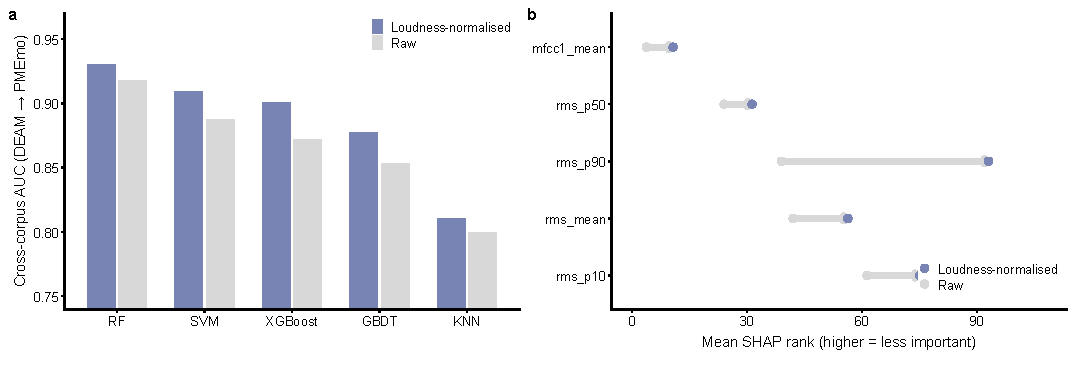
\includegraphics[width=\textwidth]{../reports/figures_r/ED1_loudness.pdf}
\caption{\textbf{Extended Data Figure 1} $|$ \legendedone}\end{figure}

\begin{figure}[p]\centering
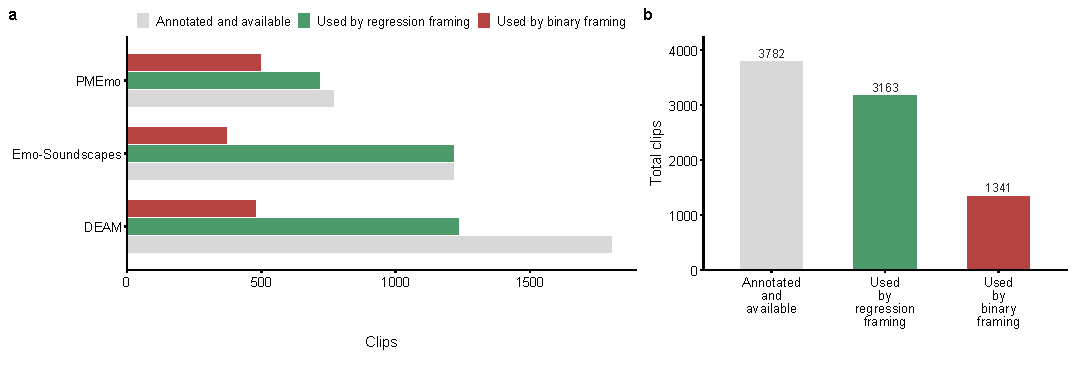
\includegraphics[width=\textwidth]{../reports/figures_r/ED2_data_use.pdf}
\caption{\textbf{Extended Data Figure 2} $|$ \legendedtwo}\end{figure}

\begin{figure}[p]\centering
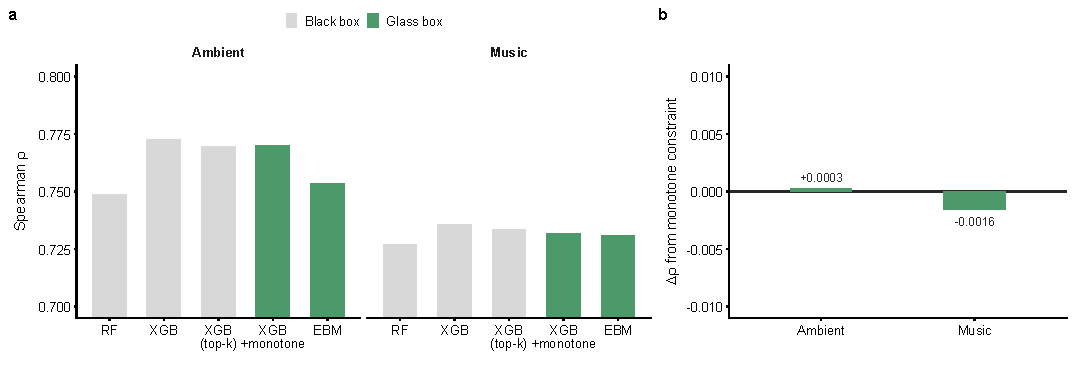
\includegraphics[width=\textwidth]{../reports/figures_r/ED3_glassbox.pdf}
\caption{\textbf{Extended Data Figure 3} $|$ \legendedthree}\end{figure}

\begin{figure}[p]\centering
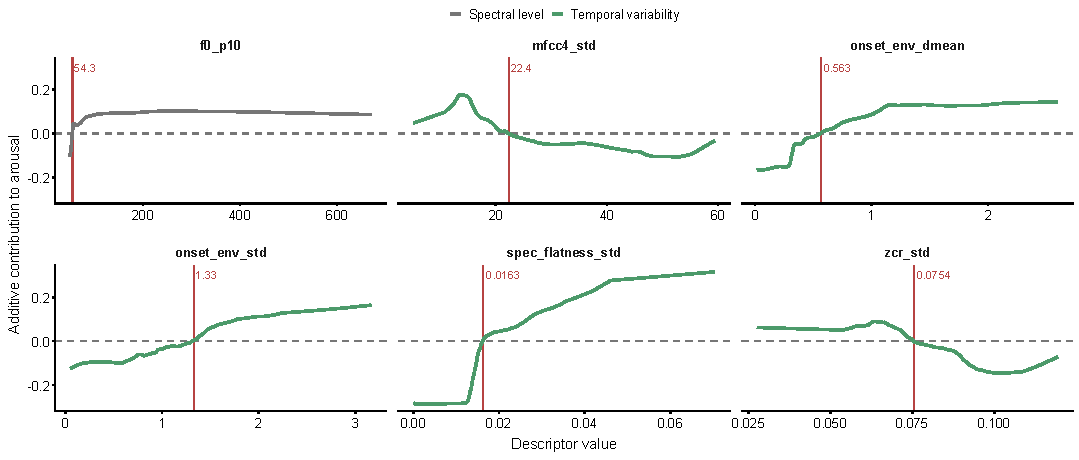
\includegraphics[width=\textwidth]{../reports/figures_r/ED4_shape_functions.pdf}
\caption{\textbf{Extended Data Figure 4} $|$ \legendedfour}\end{figure}

\begin{figure}[p]\centering
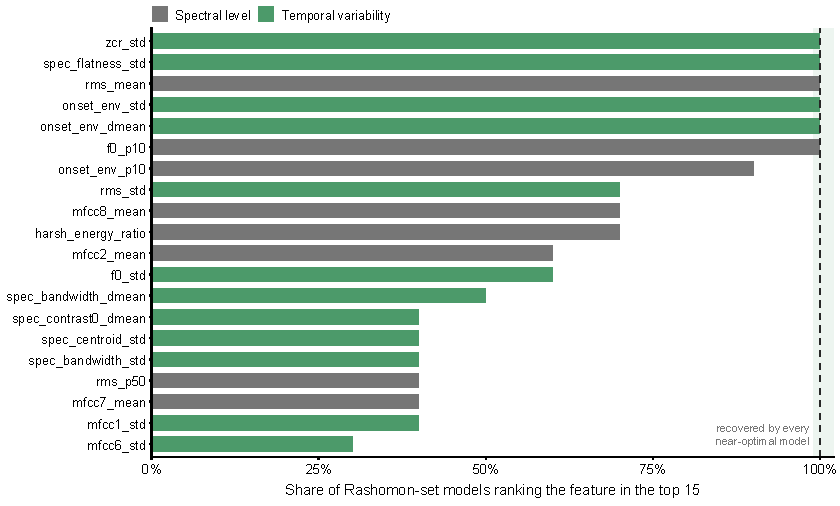
\includegraphics[width=\textwidth]{../reports/figures_r/ED5_rashomon.pdf}
\caption{\textbf{Extended Data Figure 5} $|$ \legendedfive}\end{figure}

\begin{figure}[p]\centering
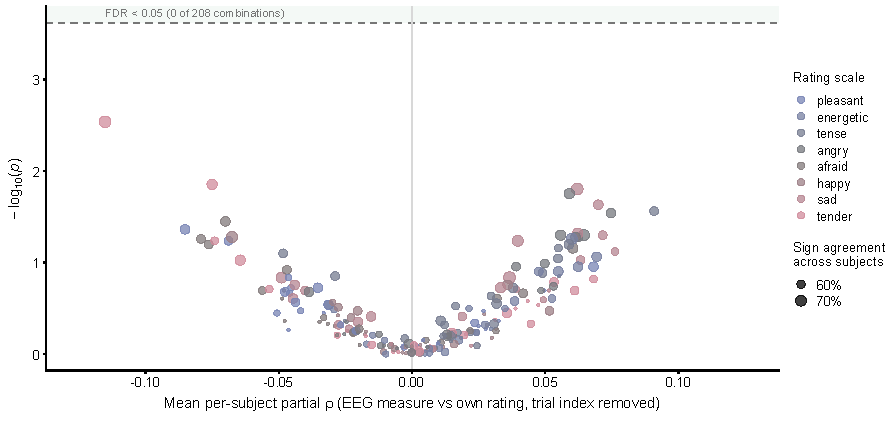
\includegraphics[width=\textwidth]{../reports/figures_r/ED6_individual.pdf}
\caption{\textbf{Extended Data Figure 6} $|$ \legendedsix}\end{figure}

\begin{figure}[p]\centering
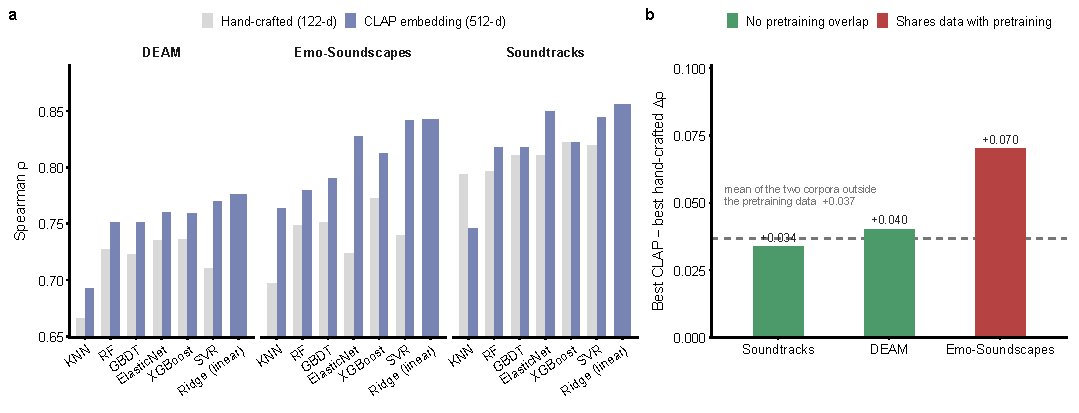
\includegraphics[width=\textwidth]{../reports/figures_r/ED7_representations.pdf}
\caption{\textbf{Extended Data Figure 7} $|$ \legendedseven}\end{figure}

\begin{figure}[p]\centering
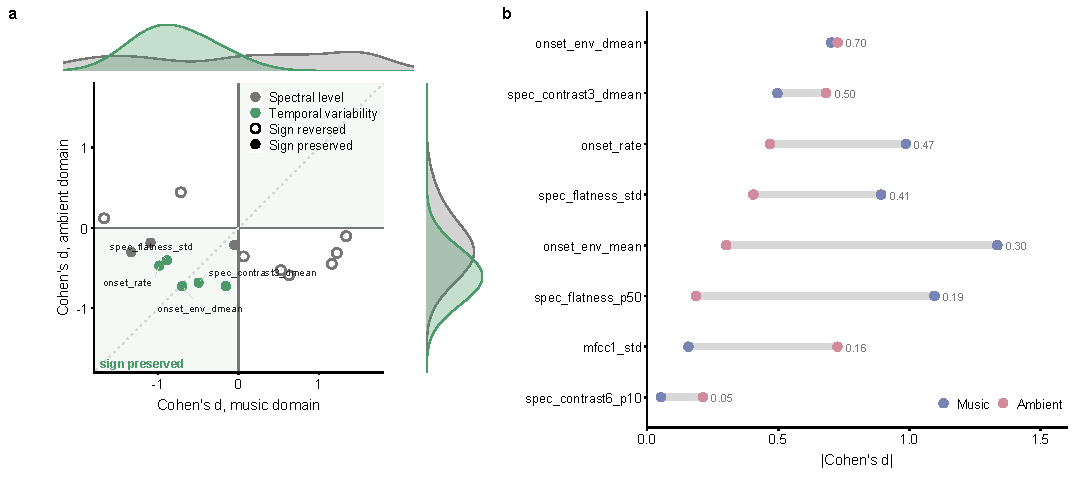
\includegraphics[width=\textwidth]{../reports/figures_r/ED8_invariance.pdf}
\caption{\textbf{Extended Data Figure 8} $|$ \legendedeight}\end{figure}

\bibliography{../references/references}

\end{document}
